\documentclass[final,12pt]{beamer}

% Setup beamerposter
\usepackage[orientation=portrait,size=a0,scale=1.75]{beamerposter} 
\usetheme{sfb1102}

% Import packages
% For image imports:
\usepackage{graphicx}
% For colored boxes, text, etc:
\usepackage{xcolor}
% Use ACL-style references:
\usepackage{acl-style-refs}
\usepackage{linegoal}

\usepackage{tikz}
\usepackage{tikz-qtree}

% Load settings and macros for the SFB poster
\usepackage{sfb-poster}
\usepackage{relsize}
\usepackage[font=footnotesize,justification=centering]{caption}
\usepackage{framed}
\usepackage{tipa}

% Fix for scaling IPA fonts
\DeclareFontFamily{T3}{cmss}{}
\DeclareFontShape{T3}{cmss}{m}{n}{%
  <-8.5> tipass8
  <8.5-9.5> tipass9
  <9.5-11> tipass10
  <11-15> tipass12
  <15-> tipass17
}{}
\DeclareFontShape{T3}{cmss}{bx}{n}{%
  <-> tipasb10
}{}
\DeclareFontShape{T3}{cmss}{m}{sl}{%
  <-> tipasi10
}{}
\DeclareFontShape{T3}{cmss}{m}{it}{%
  <-> sub * cmss/m/sl
}{}



% Macros for comments
% Inspired by Joerg Hoffman and Alvaro Torralba
\newcommand{\jutta}[1]{~\textbf{\footnotesize \color{blue} (Jutta: #1) }}
\newcommand{\vera}[1]{~\textbf{\footnotesize \color{green} (Vera: #1) }}
\newcommand{\dietrich}[1]{~\textbf{\footnotesize \color{red} (Dietrich: #1) }}


%-----------------------------------------------------------
% Name and authors of poster/paper/research
%-----------------------------------------------------------

\title{{The Effect of Prediction on Type-1 and Type-2 Language Processing}}

%\author{PIs: Vera Demberg, Jutta Kray, Dietrich Klakow }
\author{Pratik Bhandari $^{1,2,3}$ ,  David Soto $^{4,5}$ } % Author(s)

% The full institutional affiliation appears at the bottom left corner of the poster
\institute[UdS]{UdS, SFB 1102, BCBL}

% Appears centered at bottom of the poster
\footer{ICPS 2019}

% The date appears at the bottom right of the poster
%\date{17 \& 18 January 2018}
\date{07 March 2019}

%-----------------------------------------------------------
% Initiate poster
%-----------------------------------------------------------

\begin{document}
\begin{frame}[t]

\vspace{1.1em}
\begin{description}
  \item \tiny {1. Department of Psychology, Saarland University, Germany. 2. Department of Language Science and Technology, Saarland University, Germany. 3. Collaborative Research Center (SFB 1102), Saarland University, Germany}
  \centering
  \item \tiny {4. Basque Center on Cognition, Brain and Language, Spain. 5. Iquerbasque Foundation for Science, Spain}
  \centering
\end{description}

\begin{columns}[t]    
  \begin{column}{\halfpagecol}
  \vspace{-1em}
       \begin{block}{Introduction}
\vspace{-2.3cm}
\vspace{1.2em}
% \begin{greenbox}{}
\begin{itemize}
  \item Predictive processing framework: we continuously make predictions about events based on the prior probability of such occurrence $^{1}$
  \item language comprehension -- shown to operate within PP framework $^{2}$
   \item studies in low-level visual perception tasks -- stimulus predictability modulates perceptual sensitivity and metacognitive judgment $^{3}$
   \item not well-studied if such relationship extends to higher level cognitive processes like language processing
\end{itemize}
% \end{greenbox}
\end{block}
    
    
    
   \vspace{-0.15em}
   
    \begin{block}{Questions}
      \vspace{-2.3cm}
      \vspace{1.2em} %changed from 0.2em (greenbox) to 1.2em(no greenbox) -- same for all greenbox/nogreenbox throughout the poster
    % \begin{greenbox}
    
      \begin{itemize}
    \item Does animacy judgement / object categorization for predictable trials differ than that from non-predictable trials? \textit{type-1 sensitivity}
  \item Does metacognitive judgement for predictable trials differ than that from non-predictable trials? \textit{type-2 sensitivity}
  \end{itemize}
  
    % \end{greenbox}
  
   
  
    \vspace{-0.2em}
    
    \end{block}

 
   \vspace{-0.15em}
   
    \begin{block}{Predictions}
      \vspace{-2.3cm}
      \vspace{1.2em}
    % \begin{greenbox}
    
      \begin{itemize}
    \item Both type-1 and type-2 sensitivity should be higher for predictive trials than for non-predictive trials.
  \end{itemize}
  
    % \end{greenbox} 
     \vspace{-0.2em}
    
    \end{block}
    
    
    
    \vspace{-0.2em}
    \begin{block}{Methods}
    %   \textbf{\underline{Participants}}
    %   \begin{description}
    %     Within-group design
    %   \end{description}
      
        % \bigskip
        
    \begin{columns}
    \begin{column}{0.49\linewidth}
    \begin{greybox}{Participants: Group 1}
    \begin{itemize}
        \item N=16 (11 female)
        \item Age: 20-28 years {\tiny(M=22.9 yrs., SD=2)}
        \item AoA of Spanish: 0.3 years
        \item AoA of Basque: 0.8 years
        \end{itemize}
    \end{greybox}
    \end{column}
        \begin{column}{0.49\linewidth}
     \begin{greybox}{Participants: Group 2}
    \begin{itemize}
        \item N=16 (14 female)
        \item Age: 20-28 years {\tiny(M=23.5 yrs., SD=2.13)}
        \item AoA of Spanish: 0.3 years
        \item AoA of Basque: 0.9 years
        \end{itemize}
    \end{greybox}
    \end{column}
    \end{columns}    
 
     \vspace{1em}

    \begin{column}{\linewidth}
          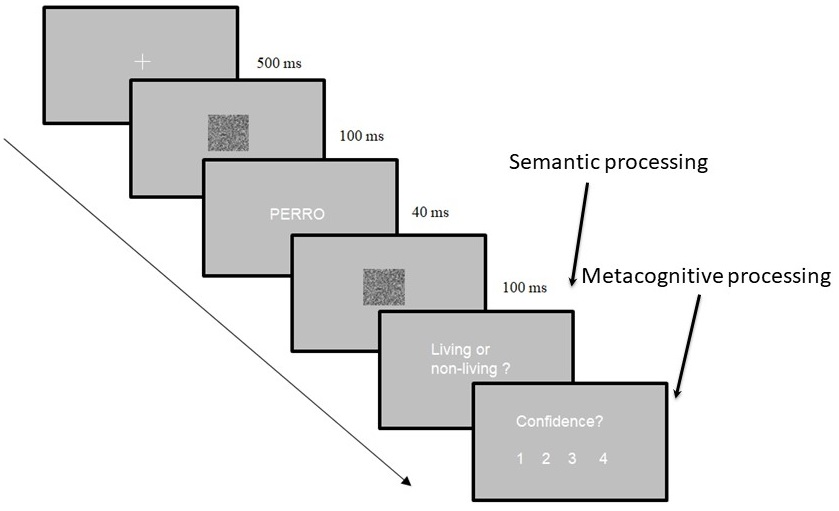
\includegraphics[width=\linewidth]{images/sampleTrial}
         \hfill
         \centering
          \scriptsize{\tiny{Fig.1: Sample trial}}
        \end{column}

\begin{columns}

     \begin{column}{0.55\linewidth}
    % \vspace{-1em}
    \begin{greybox}{Stimuli}
    {\small 640 words denoting living or non-living objects, \underline{near the threshold of awareness}}
    \begin{itemize}
        \item {\small Group 1: 'ESP predictable group'}
        \begin{itemize}
            \item {\small 80\% Spanish words,} {\tiny 20\% Basque words}
        \end{itemize}
        \item {\small Group 2: 'EUS predictable group'}
        \begin{itemize}
            \item {\small 80\% Basque words,} {\tiny 20\% Spanish words}
        \end{itemize}
        \end{itemize}
    \end{greybox}
    \end{column}


        \begin{column}{0.43\linewidth}
        % \vspace{-1em}
        \begin{greybox}{Task}
        \begin{itemize}
        \item Object categorization: {\small living or non-living}
         \item Confidence rating: {\small 1 to 4 ('guessing' to 'highly confident')}
        \end{itemize}
    \end{greybox}
    
    \end{column}


    %     \begin{column}{\linewidth}
    %       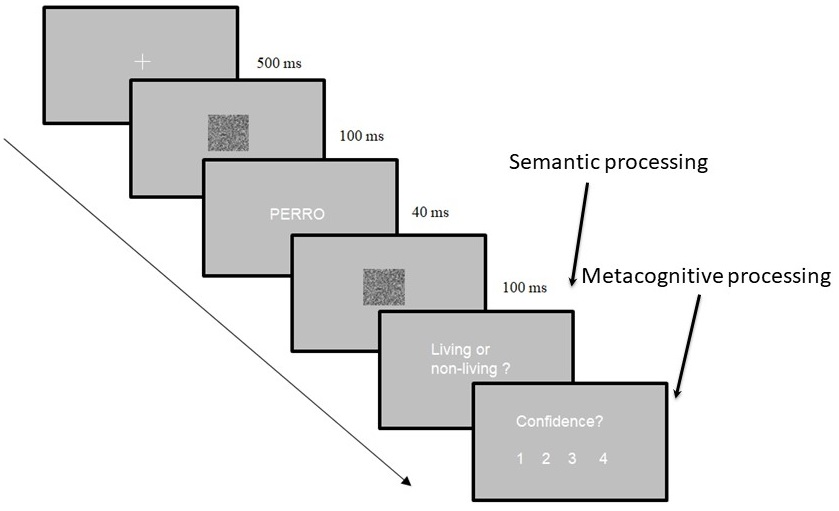
\includegraphics[width=\linewidth]{images/sampleTrial}
    %      \hfill
    %      \centering
    %       \scriptsize{\tiny{Fig.1: Sample trial}}
    %     \end{column}
      
      
      \end{columns}
      
     \end{block}
 

  \end{column}
  
%%%%%%%%%%%%%%%%%%%%%%%%%%%%%%%%%%%%%%%%%%%%%%%%%%%%%%%%%
% Second Column  
%%%%%%%%%%%%%%%%%%%%%%%%%%%%%%%%%%%%%%%%%%%%%%%%%%%%%%%%%

  \begin{column}{\halfpagecol}
  \vspace{-1em}
  \begin{block}{Results}
  \textbf{\underline{Language proficiency}}
  \begin{column}{\linewidth}
  
  \end{column}
    
  \begin{column}{\linewidth}
          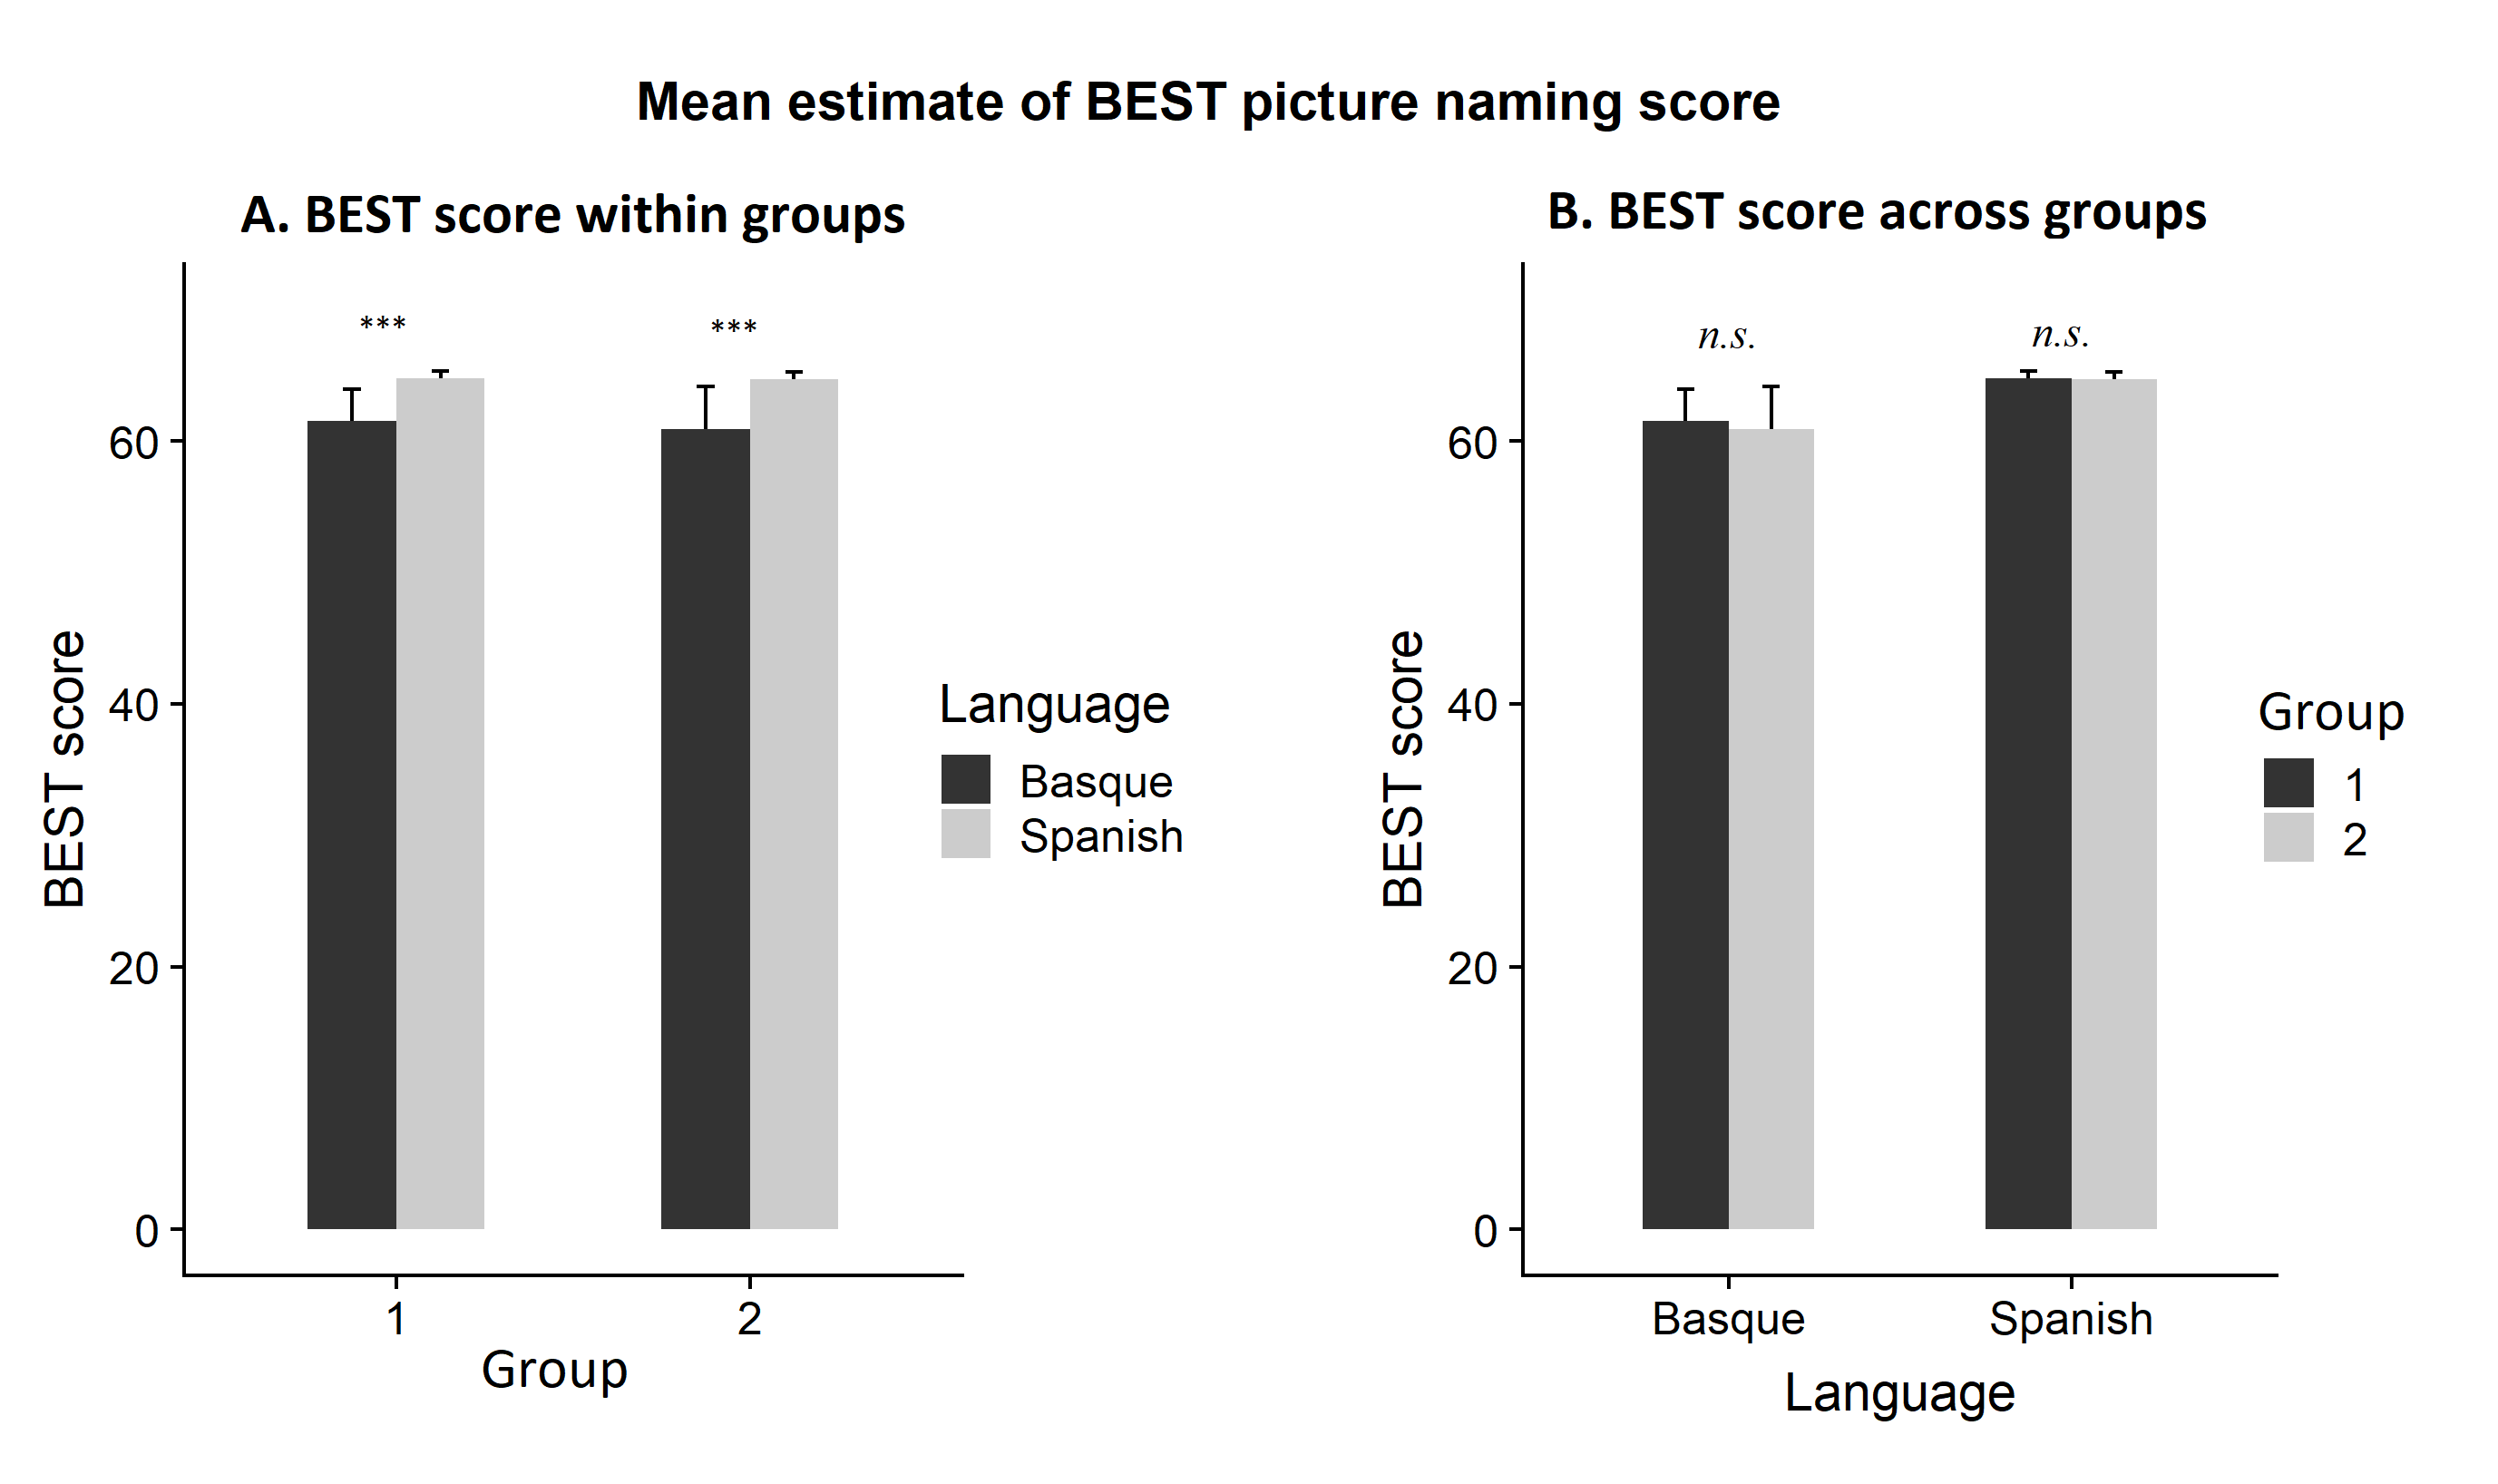
\includegraphics[width=\linewidth]{images/bestscoreplot}
          \scriptsize{\tiny{
 Fig.2: Barplot showing language proficiency scores in BEST $^{5}$ in Spanish and in Basque.
 \textbf{A.}
 Participants in both the groups had significantly higher language proficiency scores in Spanish than in Basque
 \textbf{B.} No significant difference in language proficiency scores between participants in Group 1 and Group 2 for both Spanish and Basque.
 \textit{(vertical lines represent SD from the mean. ***p\textless0.001)}}
 }
 \end{column}
  
      \vspace{1.2em}
    \textbf{\underline{Type-1 and type-2 sensitivity}}
    \begin{description}
        \item \small{Signal detection theoretic analysis $^{5}$}
    \end{description}
        \vspace{1em}

\begin{columns}

    \begin{column}{0.40\linewidth}
          \vspace{-2em}
    \begin{greybox}{}
    \begin{itemize}
        \item For Spanish trials
          \begin{itemize}
            \item {\small d': t(30) = 1.151, p=0.258}
              \item {\small meta-d': t(30) = -0.755, p=0.456}
              \end{itemize}
              \end{itemize}
             \end{greybox}
        \begin{greybox}{}
        \begin{itemize}
            \item For Basque trials
            \begin{itemize}
                \item {\small d': t(30)=3.299 , p\textless0.05}
            \item {\small meta-d': t(30)=3.791, p\textless0.001}
            \end{itemize}
            \end{itemize}
            \end{greybox}
        
    \end{column}

        \begin{column}{0.57\linewidth}
          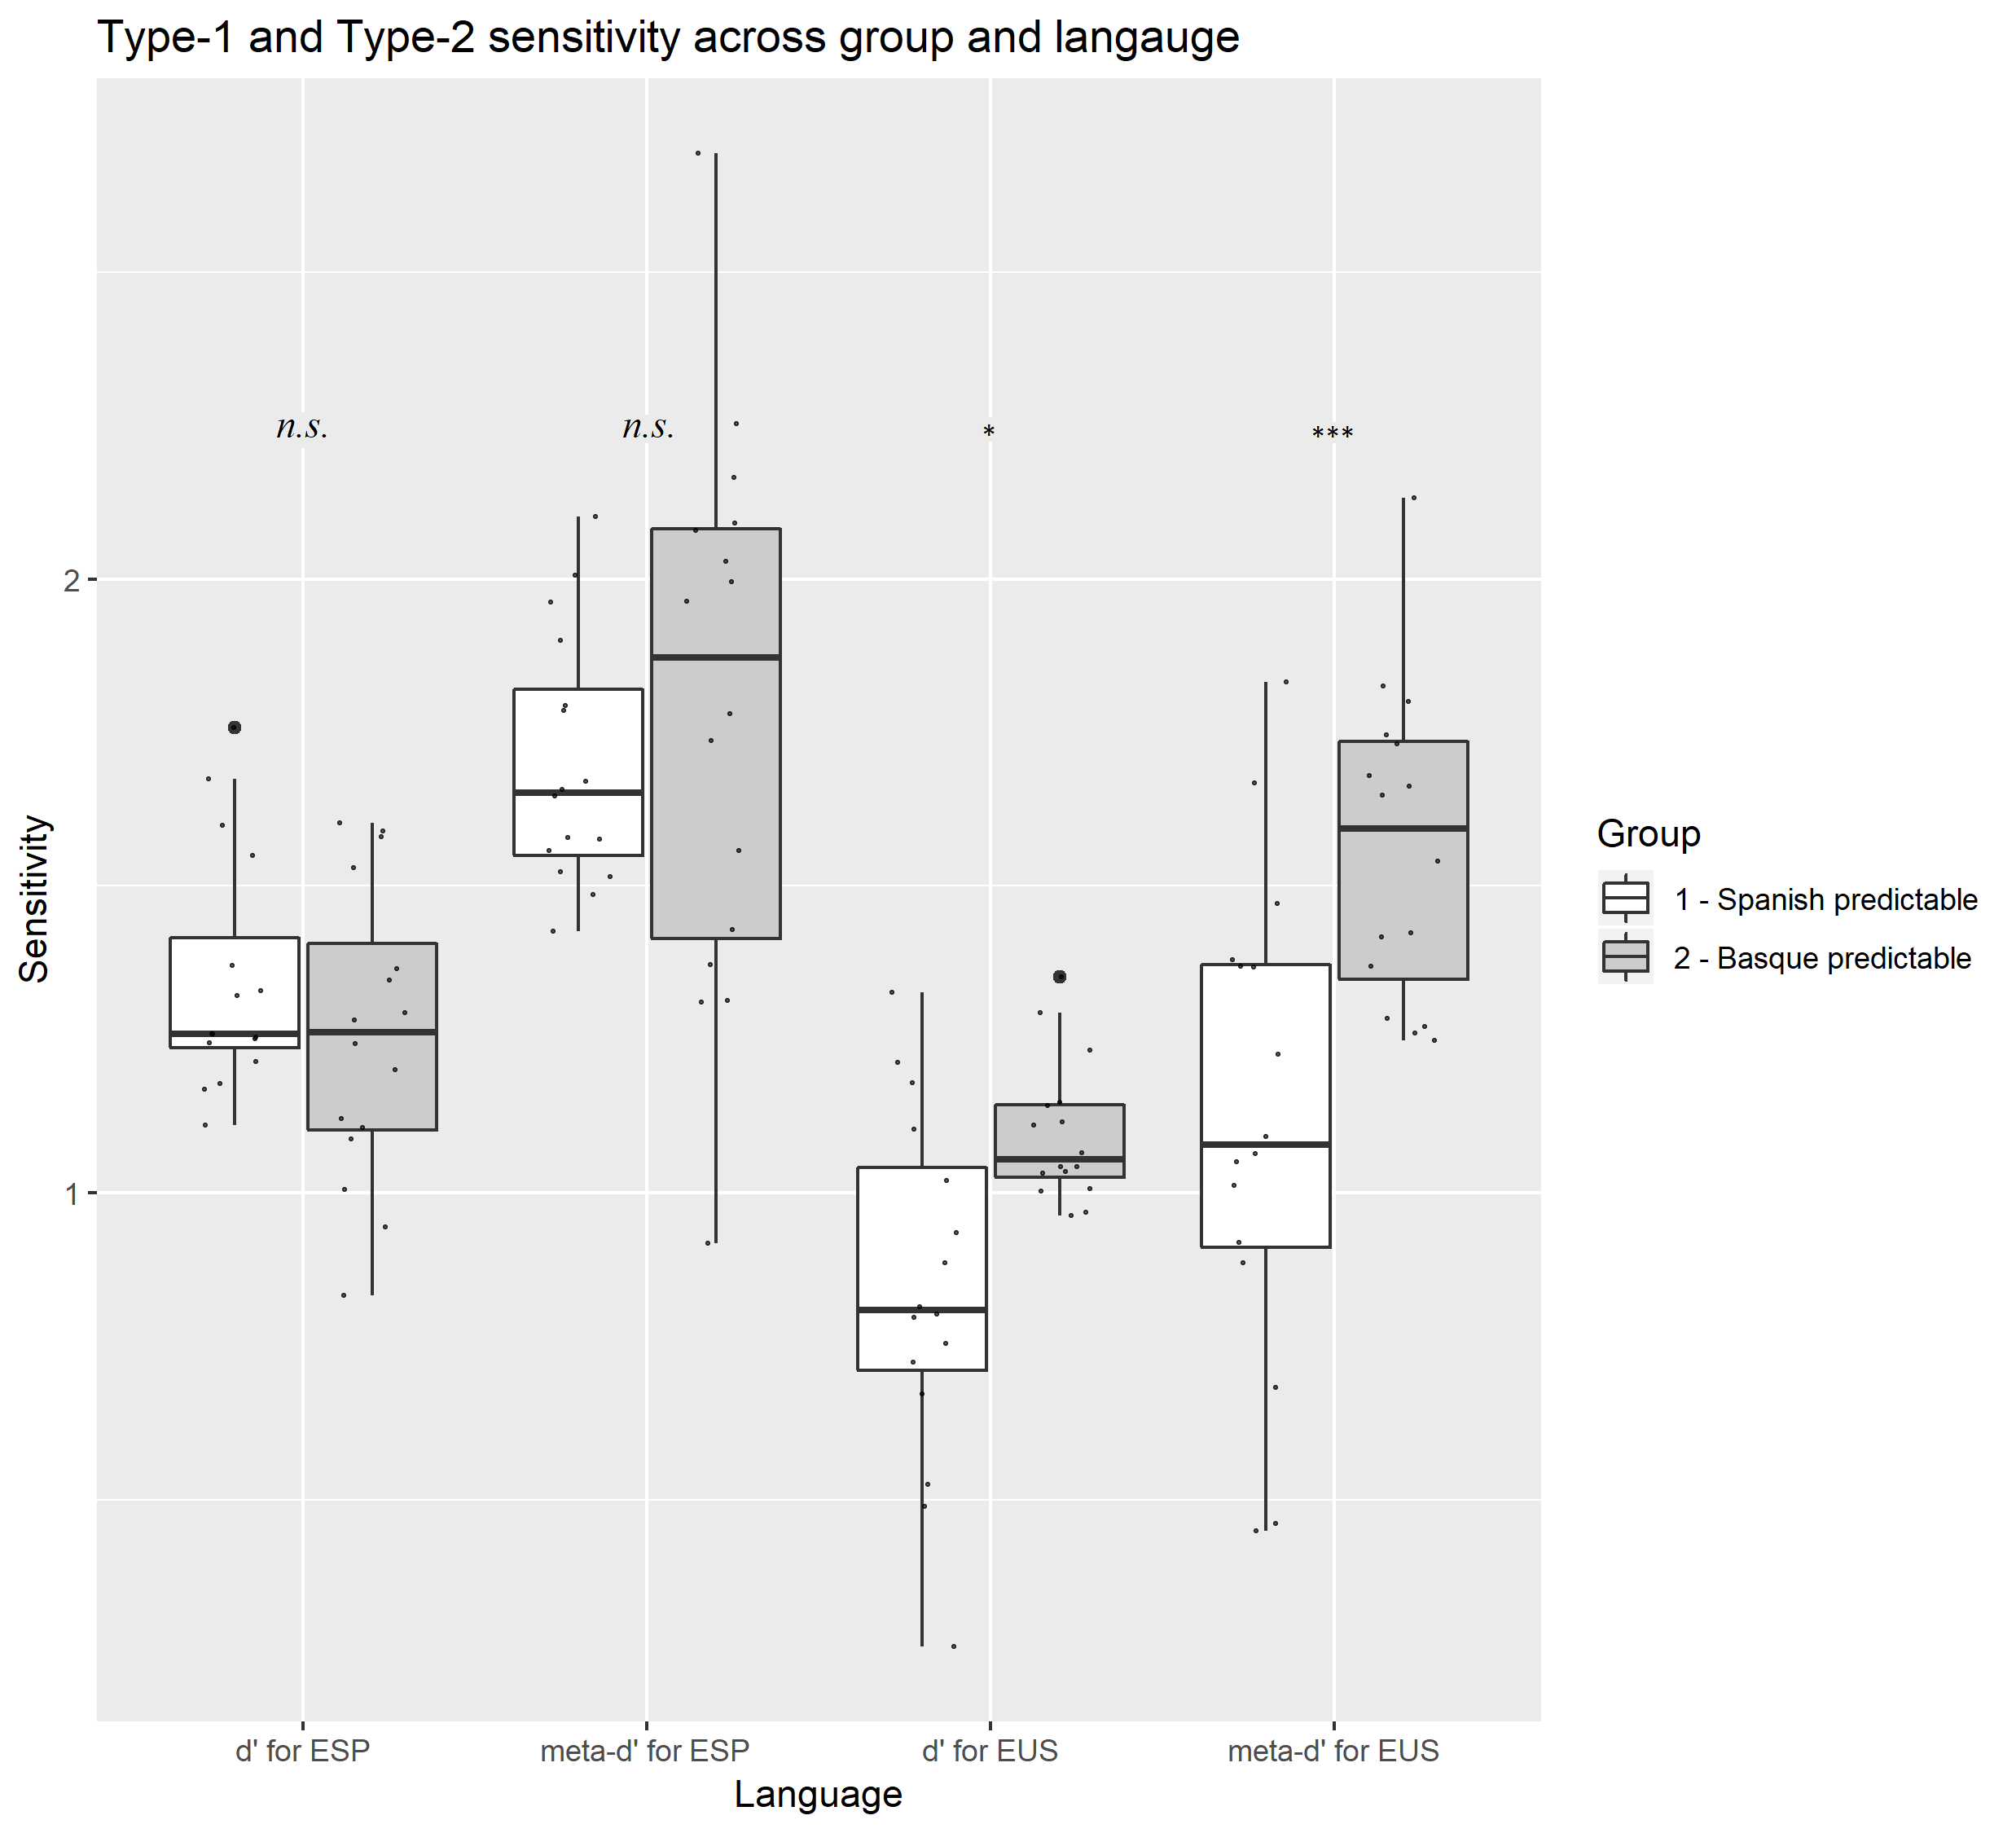
\includegraphics[width=\linewidth]{images/dmetad}
         \hfill
         \centering
          \scriptsize{\tiny{
Fig.3: Boxplot showing d' and meta-d' for trials in Spanish and in Basque for Group 1 and Group 2.
%  For Spanish trials, no significant difference in d' and in meta-d' between Group-1 and Group-2.
%  For Basque trials, both d' and meta-d' are significantly higher in Group-2 than in Group-1.
 \textit{(*p\textless0.05, ***p\textless0.001)}
 }}
        \end{column}
      \end{columns}
  
  \end{block}
  
    \vspace{-.1em}

    \begin{block}{Conclusion}
    \begin{itemize}
     \item \small Predictability enhances type-1 and type-2 language processing
     \begin{itemize}
         \item but only in low proficiency language -- \textit Basque
        \end{itemize}
    \item \small Predictability confers no processing advantage in high proficiency language \emph{(Spanish)}
%     \begin{itemize}
%         \item performance is already in ceiling
%     \end{itemize}
 \end{itemize}
 
 \begin{greybox} {Abbreviations used:}
   \begin{description}
     \item \small AoA: Age of Acquisition. ESP: Spanish. EUS: Basque
     \item \small BEST: Basque, English and Spanish Tests
   \end{description}
   \end{greybox}
    
    \end{block}
    
    

    \begin{block}{References}
    \begin{description}
     \item \small1. Clark, A. (2013). \textit{Behavioral and Brain Sciences}
    %  \item \small2. Kuperberg \& Jaeger (2015). \textit{Journal of Neuroscience}
     \item \small2. Lupyan \& Clark (2015). \textit{Curr. Dir. Psychol. Sci}
     \item \small3. Sherman et al. (2015). \textit{Consciousness and Cognition}
      \item \small4. de Bruin, Carreiras \& Dunabeitia (2017). \textit{Frontiers Psych.}
     \item \small5. Maniscalco \& Lau (2014). \textit{Cog. Neuro. Metacog.}
    \end{description}
    \end{block}
    
        \vspace{-0.8em}

   
   
    \begin{bluebox}{{\small Lets chat more!}}
    \begin{columns}

\begin{column}{0.20\linewidth}
          
\includegraphics[scale=0.5]{images/twitterqrcode}
          \centering
    \end{column}

    \begin{column}{0.56\linewidth}
         \begin{description}
        \item {\small\textit{@neurofreakPB}}
         \item {\small\texit{pratik.bhandari.np@gmail.com}}
    \end{description}
    \end{column}
    
    \begin{column}{0.20\linewidth}
          
\includegraphics[scale=0.5]{images/siteqrcode}
    \end{column}
    \end{columns}
    \end{bluebox}
    
  \end{column}
  
\end{columns} 

\end{frame}
\end{document}